% This is samplepaper.tex, a sample chapter demonstrating the
% LLNCS macro package for Springer Computer Science proceedings;
% Version 2.20 of 2017/10/04
%
\documentclass[runningheads]{llncs}
%
\usepackage{graphicx}
% Used for displaying a sample figure. If possible, figure files should
% be included in EPS format.
%
% If you use the hyperref package, please uncomment the following line
% to display URLs in blue roman font according to Springer's eBook style:
% \renewcommand\UrlFont{\color{blue}\rmfamily}

\begin{document}
%
\title{Context-Free Methods for Long-tailed Chinese Ancient Text Recognition \thanks{Supported by organization x.}}

%
%\titlerunning{Abbreviated paper title}
% If the paper title is too long for the running head, you can set
% an abbreviated paper title here
%

\author{
    Xinming Zhang\inst{1} \and
    Second Author\inst{1} \and
    Third Author\inst{1,2}
}

\authorrunning{Zhang et al.}
% First names are abbreviated in the running head.
% If there are more than two authors, 'et al.' is used.
%
\institute{
    Princeton University, Princeton NJ 08544, USA \and
    Springer Heidelberg, Tiergartenstr. 17, 69121 Heidelberg, Germany
    \email{lncs@springer.com}\\
    \url{http://www.springer.com/gp/computer-science/lncs}
}
%
\maketitle % typeset the header of the contribution


\begin{abstract}
    Long-tailed problem has been a long-standing research topic in computer vision. However, there still exists two main challenges in research of Chinese ancient text recognition task: 1) the context information significantly influences the performance of models on long-tailed datasets.  2) many existing methods lack evaluation methods specifically designed for long-tail datasets. In this paper, a context-independent data augmentation method has been proposed, which effectively alleviates the long-tail problem of ancient text recognition. This method is applied to a framework, De-ContextNet, and significantly improve model performance especially in tailed part of datasets. Specifically, words of varying lengths in a same batch are randomly concatenated together. Then the model will learn a robust representation. Furthermore, we proposed a formula for evaluating the performance of a model on long-tail datasets. Extensive experiments on three challenging Chinese ancient book datasets (TKH, MTH1000 and MTH1200) verify that our method achieves the state-of-the-art performance.\cite{zhouEastEfficientAccurate2017,zhuFourierContourEmbedding2021}
    \keywords{Open-set \and text recognition \and de-context.}
\end{abstract}
    

\section{Introduction}





% !TeX root = ../paper.tex
\section{Related Work}
% 为了排版的需要,将第3节的主图放到这里,以便图片生成时可以排在第二页
\begin{figure}
    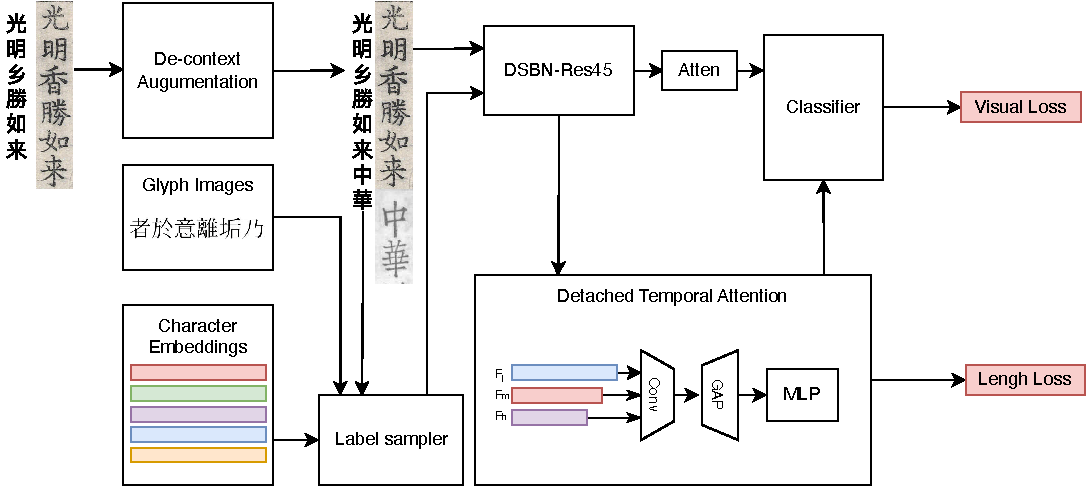
\includegraphics[width=\textwidth]{figure/paper-overall.drawio.pdf}
    \caption{A figure caption is always placed below the illustration.
    Please note that short captions are centered, while long ones are
    justified by the macro package automatically.} 
    \label{fig:overall}
\end{figure}


% 引用文献设置
\bibliographystyle{splncs04}
\bibliography{ref/refs}
% 文档结束
\end{document}
